\documentclass[conference]{IEEEtran}
\IEEEoverridecommandlockouts
% The preceding line is only needed to identify funding in the first footnote. If that is unneeded, please comment it out.
\usepackage{cite}
\usepackage{amsmath,amssymb,amsfonts}
\usepackage{algorithmic}
\usepackage{graphicx}
\usepackage{textcomp}
\usepackage{xcolor}
\def\BibTeX{{\rm B\kern-.05em{\sc i\kern-.025em b}\kern-.08em
    T\kern-.1667em\lower.7ex\hbox{E}\kern-.125emX}}
\begin{document}

\title{Parallel Matrix Multiplication\\
}

\author{\IEEEauthorblockN{Luca Falasca}
\IEEEauthorblockA{\textit{0334722} \\
luca.falasca@students.uniroma2.eu
}
\and
\IEEEauthorblockN{Matteo Conti}
\IEEEauthorblockA{\textit{0323728} \\
matteo.conti97@students.uniroma2.eu
}\\
}


\maketitle

\begin{abstract}
\end{abstract}

\section{Introduzione}
\subsection{Descrizione del problema}
Il progetto verte sulla realizzazione di un nucleo di calcolo per il prodotto tra due matrici, che sia quindi in grado di calcolare
$C \leftarrow C + AB$
dove A è una matrice $m \times k$ e B è una matrice $k \times n$. Per le matrici di input, si devono considerare due casi principali:
\begin{enumerate}
    \item Matrici quadrate $m = n = k$;
    \item Matrici rettangolari $m, n \gg k$; con $k = 32, 64, 128, 156$.
\end{enumerate}

\subsection{Obiettivi}

\subsection{Metriche di valutazione}
\subsection{Raccolta dei dati}
\section{MPI}
\subsection{Distribuzione dei dati}

\subsection{Analisi delle prestazioni}

\section{CUDA}
Tramite CUDA è possibile andare ad eseguire il codice parallelo su GPU.

\subsection{1 versione}
In questa versione del codice, si adotta un approccio procedurale nel quale si scansiona la matrice A riga per riga, dividendo ciascuna riga per il numero di processi di un blocco. Analogamente, la matrice B è suddivisa per il numero di processi. Successivamente, si avvia un ciclo in cui ogni processo elabora il proprio elemento della matrice A, moltiplicandolo per tutti i valori corrispondenti assegnati nella matrice B e sommandoli progressivamente per poi salvarli in un vettore in shared memory con indice pari all'id del processo. Ogni processo esegue questa operazione per tutti gli elementi della riga A che gli sono stati assegnati. A questo punto, una volta completate le elaborazioni da parte di tutti i processi, si sincronizzano e si sommano i risultati parziali ottenuti da ciascun processo mediante una funzione di reduce. Tale procedura viene ripetuta per tutte le colonne della matrice B. Si è scelto di utilizzare dei blocchi unidimensionali, dove ogni blocco si occupa di una riga della matrice A. Quindi c'è un numero di blocchi pari al numero di righe della matrice A (m). 

\begin{figure}
    \centering
    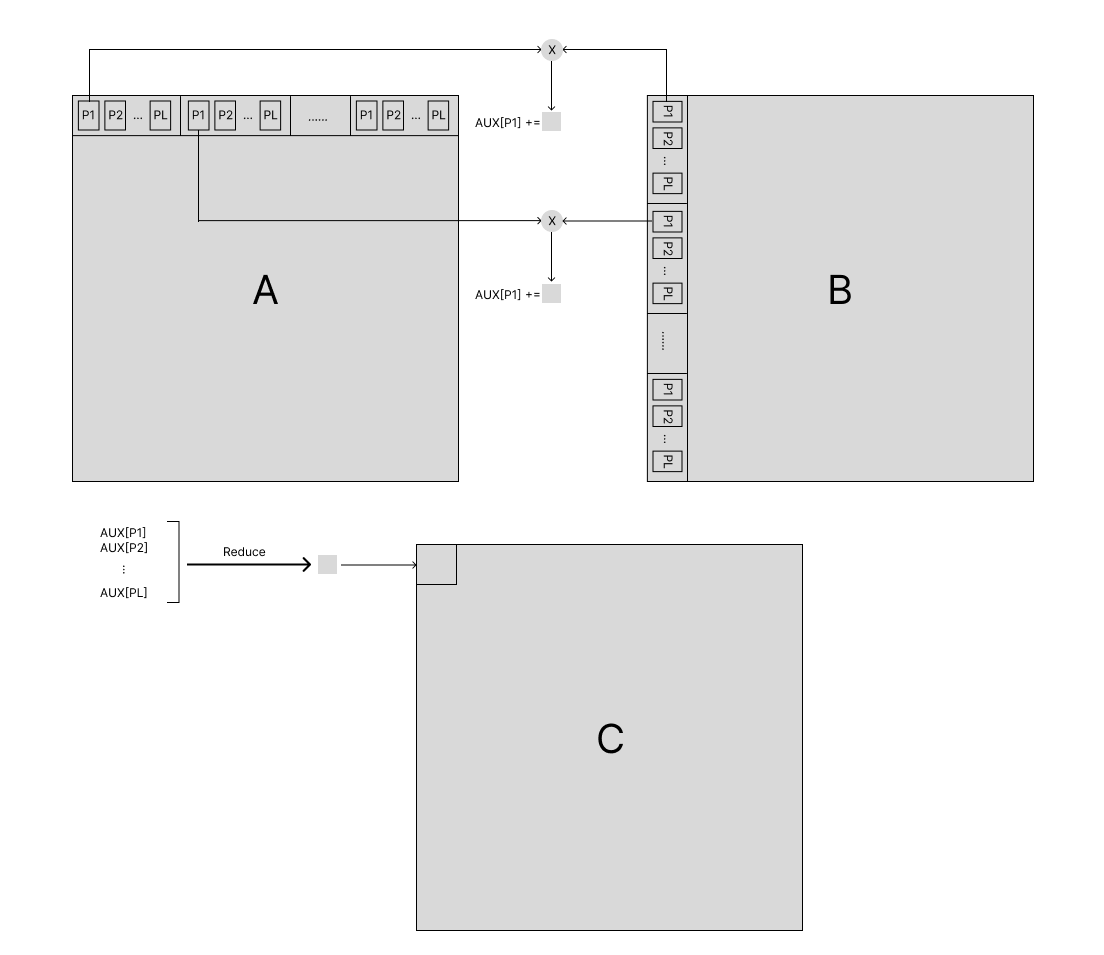
\includegraphics[width=0.5\textwidth]{resources/cuda_scheme.png}
    \caption{Schema di funzionamento della prima versione del codice CUDA.}
    \label{fig:cuda_scheme}
\end{figure}

\subsection{2 versione}
Dato che nella prima versione ad ogni iterazione sulle colonne si andava a scrivere il risultato di un solo elemento direttamente sulla matrice C, e tra la parte di calcolo e parte di reduce ci sono dei synchthreads, per ridurre l'impatto di questi synchthreads si è deciso di andare a fare un gruppo di colonne per volta e quindi scrivere i risultati parziali su una matrice temporanea in shared memory. In questo modo si riduce il numero di synchthreads che l'algoritmo deve fare 

\subsection{3 versione}
Nella terza versione si vuole sfruttare l'idea che ogni volta che si va il prodotto tra una la riga presa in considerazione e il gruppo di colonne si usano gli stessi elementi della riga A e quindi si possono salvare in shared memory. In questo modo si riduce il numero di accessi alla memoria globale e si aumenta la velocità di esecuzione. Tuttavia per come è stata fatta l'implementazione si scorre appunto una colonna per volta quindi in shared memory si dovrebbe salvare l'intera riga, ma non è auspicabile dato che la shared memory è molto limitata e le dimensioni delle righe sono molto grandi, quindi non scalerebbe bene.
Per ovviare a questo problema anzichè scorrere una colonna per volta si è deciso di scorrere la riga parziale del sottoinsieme delle colonne di B per volta. In questo modo si sfrutta la stessa porzione della riga di A per svolgere il prodotto con le colonne di B.

\subsection{4 versione}
La quarta versione è quasi equivalente alla terza, ma si applica una piccola variante al calcolo dell'indice di colonna di B. In particolare, nella versione 3
calcolo l'indice di colonna di B come $icx = i * k + j * k + ic$ dove $i$ indica la colonna in cui inizia il blocco di colonne corrente, in questo modo con $i*k$ mi posiziono all'inizio del blocco corrente, invece con j intendo l'indice della colonna corrente all'interno del blocco. In questa ulteriore versione ho semplicemente fatto un raccogliemento di $k$ in modo da ridurre il numero di moltiplicazioni portando il calcolo a $icx = (i + j) * k +ic$. Ho mantenuto queste due varianti perché nonostante sia una differenza minima crea delle differenze di performance particolari. 
\subsection{Analisi delle prestazioni}
\section{Suddivisione del lavoro}
\section*{References}

Please number citations consecutively within brackets \cite{b1}. The 
sentence punctuation follows the bracket \cite{b2}. Refer simply to the reference 
number, as in \cite{b3}---do not use ``Ref. \cite{b3}'' or ``reference \cite{b3}'' except at 
the beginning of a sentence: ``Reference \cite{b3} was the first $\ldots$''

Number footnotes separately in superscripts. Place the actual footnote at 
the bottom of the column in which it was cited. Do not put footnotes in the 
abstract or reference list. Use letters for table footnotes.

Unless there are six authors or more give all authors' names; do not use 
``et al.''. Papers that have not been published, even if they have been 
submitted for publication, should be cited as ``unpublished'' \cite{b4}. Papers 
that have been accepted for publication should be cited as ``in press'' \cite{b5}. 
Capitalize only the first word in a paper title, except for proper nouns and 
element symbols.

For papers published in translation journals, please give the English 
citation first, followed by the original foreign-language citation \cite{b6}.

\begin{thebibliography}{00}
\bibitem{b1} G. Eason, B. Noble, and I. N. Sneddon, ``On certain integrals of Lipschitz-Hankel type involving products of Bessel functions,'' Phil. Trans. Roy. Soc. London, vol. A247, pp. 529--551, April 1955.
\bibitem{b2} J. Clerk Maxwell, A Treatise on Electricity and Magnetism, 3rd ed., vol. 2. Oxford: Clarendon, 1892, pp.68--73.
\bibitem{b3} I. S. Jacobs and C. P. Bean, ``Fine particles, thin films and exchange anisotropy,'' in Magnetism, vol. III, G. T. Rado and H. Suhl, Eds. New York: Academic, 1963, pp. 271--350.
\bibitem{b4} K. Elissa, ``Title of paper if known,'' unpublished.
\bibitem{b5} R. Nicole, ``Title of paper with only first word capitalized,'' J. Name Stand. Abbrev., in press.
\bibitem{b6} Y. Yorozu, M. Hirano, K. Oka, and Y. Tagawa, ``Electron spectroscopy studies on magneto-optical media and plastic substrate interface,'' IEEE Transl. J. Magn. Japan, vol. 2, pp. 740--741, August 1987 [Digests 9th Annual Conf. Magnetics Japan, p. 301, 1982].
\bibitem{b7} M. Young, The Technical Writer's Handbook. Mill Valley, CA: University Science, 1989.
\end{thebibliography}
\vspace{12pt}


\end{document}